\uchapter{Fundamentação teórica}
\label{cap:fundamentacao-teorica}

Neste capítulo, apresentaremos os conceitos centrais que serviram como base e guia para a elaboração deste trabalho.

\section{Compilador}
Programas que são executados em computadores são escritos no que é chamada de linguagem de máquina que usa comandos simples que são interpretados pela máquina. Escrever em linguagem de máquina é uma tarefa passível de erro e cansativa, e por essa razão foram criados os compiladores. Os compiladores traduzem linguagens de alto nível em linguagem de máquina e indicam erros cometidos pelos programadores no código-fonte \cite{mogensen2024introduction}.

\subsection{Fases do compilador}
As fases de um compilador podem ser divididas de várias formas, mas para esse trabalho será seguida a definição de \textcite{thain2020introduction}. 


\begin{figure}[ht]
    \captionsetup{width=16cm}
    \Caption{\label{fig:compfases}Fases de um compilador UNIX}
    \tcbox[left=0cm, right=0cm, top=0cm, bottom=0cm,center]{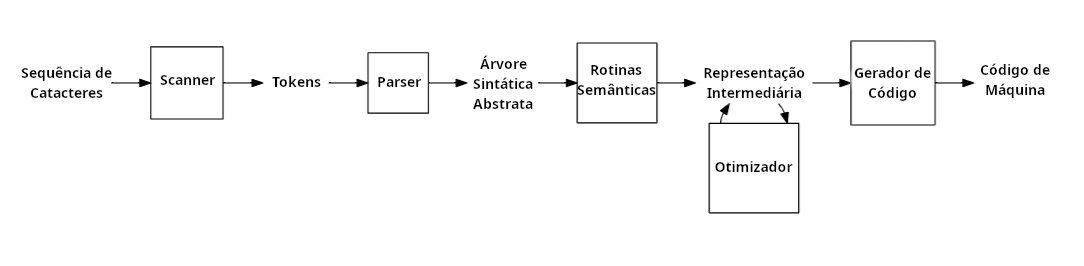
\includegraphics[width=15.6cm]{figuras/compfases.png}}{
    \Fonte{adaptada de \textcite{thain2020introduction}.}}
\end{figure}
\FloatBarrier

\subsubsection{Análise Léxica}
Na fase de análise léxica, o \textit{scanner}, também chamado de \textit{tokenizer}, consome texto simples de um programa e agrupa os caracteres individuais em sequências chamadas de \textit{tokens}. Esse processo funciona de forma parecida com agrupar letras para formar palavras da linguagem natural.

\subsubsection{Análise Sintática}
A fase de análise sintática da compilação rearranja os \textit{tokens} gerados pela fase de análise léxica, gerando assim uma estrutura chamada árvore sintática. Árvores sintáticas são estruturas de árvore como diz o nome, as folhas dessa árvore são os \textit{tokens} e a leitura em ordem da árvore dá a sequência de \textit{tokens} do texto de entrada dado ao analisador sintático. Ao construir a árvore sintática, o analisador sintático também checa se há erros de sintaxe no texto de entrada.

\subsubsection{Análise semântica}
Na fase de análise semântica, as rotinas semânticas percorrem a árvore sintática e buscam significado na entrada a partir das regras da gramática e da relação entre os elementos da entrada. Depois das rotinas semânticas, a árvore de análise sintática é convertida em uma representação intermediária que é uma versão simplificada de \textit{assembly} que permite uma análise detalhada.

\subsubsection{Otimização}
Na fase de otimização, otimizadores são aplicados na representação intermediária para tornar o programa mais rápido, menor e eficiente. Normalmente os otimizadores recebem uma entrada em formato de representação intermediária e retornam um resultado no mesmo formato para que todos os otimizadores possam ser aplicados de forma independente e em qualquer ordem.

\subsubsection{Geração de código}
Na fase de geração de código, o gerador de código consome a representação intermediária otimizada e a transforma em um programa em \textit{assembly} concreto. Para otimizar o uso dos registradores físicos limitados e gerar instruções de montagem de maneira eficiente, o gerador de código precisa executar as tarefas de alocação de registradores, seleção de instruções e sequenciamento de instruções.

\section{Analisadores Sintáticos Descendentes}
Analisadores sintáticos descendentes, também chamados de \textit{parsers top-down}, são métodos de análise sintática que iniciam a análise a partir do símbolo inicial da gramática, eles fazem comparações entre os \textit{tokens} do texto de entrada e os símbolos da gramática para encontrar a produção que deve ser escrita no lugar dos símbolos da gramática, essas comparações são feitas até sobrar apenas símbolos terminais, esses símbolos terminais devem coincidir com a sequência de \textit{tokens} da entrada caso contrário será considerado um erro.

\subsection{Descendentes Recursivos}
O conjunto de gramáticas que pode ser analisados usando algoritmos usando apenas um não terminal e o próximo símbolo da entrada é chamado de gramáticas LL(1). Uma das formas de fazer a análise dessas gramaticas é usando o analisador sintático descendente recursivo que usa funções recursivas para cada não terminal para processar a entrada. É um algoritmo que funciona como uma forma recursiva dos analisadores sintáticos LL(1) além de não seguirem estruturas fixas e determinísticas e por isso não será abordado na ferramenta.

\subsection{Analisadores Sintáticos LL(1)} 
% \ctext[RGB]{180, 250, 180}{Escrever mais detalhado sobre LL(1)} \newline
Analisadores sintáticos LL(1) são um tipo de analisador sintático descendente, esse analisador sintático leva em consideração um \textit{lookahead} que nesse algoritmo é o símbolo inicial do lado direito das produções, o \textit{lookahead} é usado para decidir qual produção deve ser escrita, por essa razão apenas gramaticas não ambíguas podem ser analisadas pelos analisadores sintáticos LL(1).

O conjunto dos símbolos iniciais das produções de uma gramática é chamado conjunto \textit{first}, a construção desse conjunto pode ser feita seguindo o Algoritmo \ref{alg:first}. As definições dos algoritmos foram tiradas do trabalho de \textcite{thain2020introduction}.


\begin{algorithm}[htp]
    \caption{First}\label{alg:first}
    \Input{Gramática G, simbolo X }
    \Output{Conjunto first}
    first = $\{\}$\\
    \Inicio{
        \Switch{X}{
            \Case {Terminal}{
                first = \{X\}
            } 
            \Casex{Não terminal}{
                \Repeat{não haja mais mudanças}{
                    \ForEach{regra $X \rightarrow Y_1Y_2...Y_k$ na Gramática G}{
                        \Ifx {a está em First($Y_1$) ou a está em First($Y_n$) e $Y_1.. Y_{n-1} \Rightarrow \epsilon$} {Adicionar a ao first}            \Ifx{$Y_1...Y_k \Rightarrow \epsilon$}{
                        Adicionar $\epsilon$ ao first
                        }
                    }
                }
            }
        }
    }
\end{algorithm}


O conjunto \textit{follow} é o conjunto de símbolos terminais da gramática que podem ocorrer depois de qualquer uma das derivações de um não terminal $A$, o conjunto também inclui o símbolo $\$$ usado para se referir ao fim da \textit{string} Esse conjunto é usado no analisador LL para lidar com produções que derivam uma \textit{string} vazia. A construção do conjunto \textit{follow} pode ser feita seguindo o Algoritmo \ref{alg:follow}.

\begin{algorithm}[htp]
    \caption{Follow}\label{alg:follow}
    \Inicio{
        Follow(S) = \{\$\} onde S é o símbolo inicial.\\
        \Repeat{ até não houver mais mudanças}{
        \Ifx {A → $\alpha B \beta$ }{
        adiciona First($\beta$) (exceto $\epsilon$) ao Follow(B).}
        \Ifx {A → $\alpha B$ ou First($\beta$) contém $\epsilon$} {
        adiciona Follow(A) ao Follow(B).}
        }
    }
\end{algorithm}
\FloatBarrier

Uma tabela de análise sintática LL(1) pode ser usada para determinar as regras a serem usadas na análise de uma trada para todas as combinações de não terminais e \textit{tokens} da entrada. A construção dessa tabela pode ser feita usando os conjuntos de \textit{first}e \textit{follow}usando o Algoritmo \ref{alg:lltable}.

\begin{algorithm}[htp]
    \caption { Construção da tabela LL(1)}\label{alg:lltable}
    
    \Input {Grammar G}
    \Output {Parsing table M }
    \Inicio{
        \ForEach {regra A $\rightarrow \alpha$ em G} {
            \ForEach {terminal $a$ (exceto $\epsilon$) em First($\alpha$)} {
                adiciona A $\rightarrow \alpha$ a $T [A, a]$.}
            \Ifx {$\epsilon$ está em First($\alpha$)}
                {\ForEach {terminal b (incluindo \$) em Follow(A)}{
                adiciona A $\rightarrow \alpha$ to $T [A, b]$.}}
        }
    }
\end{algorithm}
\FloatBarrier

Tendo a tabela de análise sintática LL(1) em mãos, é possível fazer a análise de uma sequência de \textit{tokens} usando uma \textit{stack}. O Algoritmo \ref{alg:lltparse} mostra a análise sintática usando a tabela. 

\begin{algorithm}[htp]
\caption{Analise com tabela LL(1)}\label{alg:lltparse}
\Input{Gramática G com simbolo inicial P, tabela T}
\Inicio{
    cria uma stack S.\\
    monta \$ e P em S.\\
    token c = o primeiro token na entrada.\\
    \While {S não está vazio} {
        token X = o topo de S. \\
        \Ifx {X faz par com c} {
            remova X de S.\\
            avança c para o proximo token\\
            repetir.}
        \Ifx {X é um terminal} {para com um erro.}
        \Ifx {T [X, c] aponta para a regra $X \rightarrow \alpha$}{
            remova X de S.\\
            monta os símbolos $\alpha$ em S.\\
            repetir.}
        \Ifx {T [X, c] aponta para um estado de erro} {para com um erro.}
    }
}
\end{algorithm}
\FloatBarrier

\section{Analisadores Sintáticos Ascendentes}
Os analisadores sintáticos ascendentes levam uma abordagem oposta aos analisadores sintáticos descendentes. Ao invés de começar com o símbolo inicial da gramática, os analisadores sintáticos ascendentes procuram sequências de \textit{tokens} que façam par com o lado direito das produções da gramática e substituem as sequências de \textit{tokens} pelo símbolo não terminal do lado esquerdo da produção. Esse processo é repetido até que toda a sequência de \textit{tokens} seja reescrita e apenas reste o símbolo inicial da gramática.

\subsection{Analisadores Sintáticos SLR}

Há um conjunto de gramáticas que podem ser analisadas usando técnicas de \textit{shift-reduce} e um único \textit{lookahead}, esse conjunto de gramáticas pode ser chamado de LR(1). As ações de \textit{shift-reduce} são usadas para reduzir \textit{tokens} de uma entrada a não terminais, quando uma sequência de \textit{tokens} pode ser reduzida ao símbolo inicial da gramática a análise da entrada teve sucesso, caso contrário há um erro na entrada.

Todas as ações de \textit{shift-reduce} possíveis podem ser calculadas para uma gramática construindo um autômato LR(0), que também pode ser chamado de coleção de itens canônicos. Esse autômato guarda todas as possíveis posições de leitura das produções da gramática representadas por um ponto escrito no lado direito das produções.

As ações de \textit{shift-reduce} são definidas pelas transições do autômato e pela posição de leitura, caso uma transição seja feita com um terminal a ação será de \textit{shift}, caso uma transição seja feita com um não terminal a ação será de \textit{goto}, caso a posição de leitura esteja no fim da produção a ação será de \textit{reduce}. 

O Algoritmo \ref{alg:automaton} mostra como construir o autômato LR(0) com o auxílio do \textit{closure} mostrado no Algoritmo \ref{alg:closure}.

\begin{algorithm}[ht]
    \caption{Closure}\label{alg:closure}
    \Input{Gramática G, Estado S}
    \Inicio{
        \Repeat{não tenha itens a serem adicionados}{ 
            \ForEach {item da forma $A \rightarrow \alpha .X \beta$ em S com $X \in NT$ } {
                \ForEach{produção da forma $X \rightarrow \gamma $ em G}{
                    adiciona uma produção da forma $X \rightarrow .\gamma$ a S
                }
            }
        }
    }
\end{algorithm}
\FloatBarrier

Quando um símbolo não terminal produz um símbolo terminal, apenas um caminho para derivação é possível, já que um não terminal não pode ser derivado, no entanto, quando um não terminal produz outro não terminal, o não terminal produzido terá outras derivações, por isso é preciso levar em consideração as produções dos não terminais que estão sob a posição de leitura dentro da produção de outro não terminal, \textit{closure} é o nome dado a ação de completar os estados do autômato adicionando essas produções. 

\begin{algorithm}[ht]
    \caption{Construção do autômato LR(0)}\label{alg:automaton}
    \Input{Gramática G}
    \Output{Autômato LR(0)}
    \Inicio{
        cria um autômato m \\
        estado s0 = \{P | para a produção do símbolo inicial $A \rightarrow \gamma$, P é uma produção da forma $A \rightarrow .\gamma$ \}.\\
        closure(s0)\\
        adiciona s0 a m\\
        conjunto de estados newStates = \{s0\} \\
        \ForEach{estado s em newStates} {
            conjunto de estados temp = \{\}\\
            \ForEach{símbolo a em $T\cup NT$}{
                estado s1 = \{\}\\
                \ForEach{produção da forma $A \rightarrow \alpha . a \beta$ em s}{
                    adiciona uma produção da forma $A \rightarrow \alpha a. \beta$ em s1\\
                }
                
                closure(s1)\\
                
                \Ifx{s1 não está em m}{
                    adiciona s1 a m\\
                    adiciona a transição $\hat{\delta}(s, a)=\hat{\delta}(s, a)\cup\{s1\}$ a m\\
                    adiciona s1 a temp
                }
            }
            newStates = temp
        }
        \Return{m}
    }
\end{algorithm}
\FloatBarrier 

Usando o autômato LR(0) podemos construir uma tabela de ações e \textit{goto} para facilitar o acesso a essas informações durante o processo de análise sintática. Essa pode ser calculada usando o Algoritmo \ref{alg:slrtable}.

A análise sintática do analisador sintático SLR pode ser feita usando a tabela de ações e \textit{goto} seguindo o Algoritmo \ref{alg:slrparsing}.
\begin{algorithm}[htp]
    \caption{Construção da tabela SLR}\label{alg:slrtable}
    \Input{Autômato LR(0)}
    \Inicio{
        tabela ACTION\\
        tabela GOTO\\
        \ForEach {estado s} {
            \ForEach {item da forma $A \rightarrow \alpha . a \beta$}{
                ACTION[s, a] = shift para o estado t de acordo com o autômato LR(0).}
            \ForEach {item da forma $A \rightarrow \alpha . B \beta$}{
                GOTO[s, B] = goto para o estado t de acordo com o autômato LR(0).}
            \ForEach {item da forma $A \rightarrow \alpha .$}{
                \ForEach{ terminal a em FOLLOW(A)}{
                    ACTION[s, a] = reduce pela regra $A \rightarrow \alpha$
                }
            }
        }
        Todos os estados restantes são estados de erro.
    }
\end{algorithm}
\FloatBarrier

\begin{algorithm}[htp]
    \caption{Analise com tabela SLR}\label{alg:slrparsing}
    \Input{Tabela de ações ACTION, Tabela goto GOTO}
    \Inicio{
        stack de estados S.\\
        monta S0 em S.\\
        token a = primeiro token da entrada.\\
        \While{verdade}{
        estado s = topo de S.\\
        \If {ACTION[s, a] for aceite}{
        analise completa.}
        \ElseIf {ACTION[s, a] for shift t}{
        monta estado t em S.\\
        token a = próximo token da entrada.}
        \ElseIf {ACTION[s, a] for reduce $A \rightarrow \beta$}{
        desmonta estados correspondentes a $\beta$ de S.\\
        estado t = topo de S.\\
        monta GOTO[t, A] em S.}
        \Elsex{
        para com um erro.}
        }
    }
\end{algorithm}
\FloatBarrier

\subsection{Analisadores Sintáticos CLR}
O analisador sintático \textit{canonical} LR (CLR) é um analisador sintático descendente para gramáticas LR(1). O analisador sintático CLR usa o autômato LR(1) para construção da tabela de ações e \textit{goto}, esse autômato é parecido com o autômato LR(0), o que diferencia os dois é que todos os itens do autômato LR(1) tem uma anotação do conjunto de \textit{tokens} que podem aparecer depois desses itens. Esse conjunto é chamado de \textit{lookahead}. 

A construção do autômato LR(1) segue o mesmo algoritmo da construção do autômato LR(0) com algumas modificações. A primeira produção a ser adicionada no primeiro estado do autômato vai ser adicionada com o \textit{lookahead}, esse \textit{lookahead} tem $\$$ como único elemento. Ao computar o \textit{closure} serão considerados dois casos:
\begin{itemize}[label=$\sbullet$]
    \item Para produções da forma $A \rightarrow \alpha . B $ com \textit{lookahead} de $\{L\}$, deverão ser adicionadas novas produções da forma $B \rightarrow . \gamma$ com \textit{lookahead} de $\{L\}$
    \item Para produções da forma $A \rightarrow \alpha.B\beta$, com \textit{lookahead} de $\{L\}$, deverão ser adicionadas novas produções da forma $B \rightarrow . \gamma$ com \textit{lookahead} da seguinte forma:
    \begin{itemize}
        \item Se $\beta$ não produz $\epsilon$, o \textit{lookahead} é $First(\beta)$.
        \item Se $\beta$ produz $\epsilon$, o \textit{lookahead} é $First(\beta)\cup\{L\}$.
    \end{itemize}
\end{itemize}

\section{Learning Tools Interoperability}
Learning Tools Interoperability (LTI) em português interoperabilidade de ferramentas de aprendizagem é um padrão técnico desenvolvido pela 1EdTec\footnote{https://www.1edtech.org/}. Esse padrão especifica métodos de comunicação entre Learning Management System (LMS) em português sistema de gerenciamento de aprendizagem e ferramentas de aprendizagem remotas \cite{1edtech}.

LTI permite a implementação das seguintes funcionalidades:
\begin{itemize}[label=$\sbullet$]
    \item Assignment and Grade Services (AGS) que fornece uma maneira de criar uma coluna de boletim de notas e publicar notas associadas a um link de recurso.
    \item Names and Role Provisioning Services 2.0 (NRPS) que fornece acesso a dados sobre usuários e suas funções nas organizações; uma escola, plataforma (LMS) ou curso são exemplos de organização.
    \item Deep Linking 2.0 (DL) que permite que um professor ou usuário de plataforma (LMS) integre conteúdo coletado de uma ferramenta externa. Usando este serviço, os usuários da plataforma podem lançar um URI especificado pelo fornecedor do currículo digital (ferramenta externa), selecionar conteúdo específico e, em seguida, receber um URI que outros usuários podem usar para lançar diretamente esse conteúdo.
\end{itemize}